\subsection{Electrically Small Radiating Sources in TEM Cells}

% What is this subsection for? Maybe it should be combined with the TEM cell section. In there, the calculations with Green's theorem and Lorentz Reciprocity Theorem could be put. Then, the calculations from the paper of Sreenivasia could follow. It shows how to find the equivalent Dipole moments. It is important to know which modes are propagating. A Electric dipole, which points in direction of wave propagation, should not influence the result. However, it could create TM modes, which would transfer power to the ports. -> Investigate modes.

An electrically small radiating source may be represented by six dipoles. This number includes three magnetic dipoles pointing in every direction of the Cartesian coordinate system (x, y, and z-direction), and three electric dipoles in the same orientation. Consequently, an equipment under test (EUT) could be modeled with these dipoles, leading to much less computational effort in simulation. The excited EM waves by point sources is discussed in \cite{Collin_2015} and in \autoref{sec:modes_tem_cell}. An analytical procedure to determine these dipole moments is presented by Sreenivasiah \cite{Sreenivasiah_Chang_Ma_1981}, and some experimental results based on it can be found in the research of Kreindl, where bond wires were modeled with magnetic dipoles\cite{Kreindl_Bauernfeind_Weiss_Stockreiter_Kaltenbacher_2024}, and, again, Sreenivasiah \cite{Sreenivasiah_Chang_Ma_1981}.

% Citing: "If the waveguide walls are perfectly conducting, the coefficients of such an expansion may be obtained in a straightforward manner, by an application of Lorentz's reciprocity principle." - This should be treated in the section about TEM cells. A reference to the Lorentz Reciprocity Theorem shall be made, and how it is used to determine the coefficients of the orthonormal modes.

The idea is to place the EUT in the TEM cell and measure the power of both output ports. The amplitudes of the TEM fields are expressed by \autoref{eqn:a_b_moments} \cite{Sreenivasiah_Chang_Ma_1981}. % maybe cut out this equation.

\begin{equation}
    \begin{pmatrix}a \\b\end{pmatrix} = \frac{1}{2}(-\mathbf{m_e}\cdot \mathbf{E_0}^\pm+\mathrm{i}\omega\mu_0\mathbf{m_m}\cdot\mathbf{H_0}^\pm)
    \label{eqn:a_b_moments}
\end{equation}

The magnetic field $\mathbf{H_0}$ and electric field $\mathbf{E_0}$ are both normalized to $1\,\sqrt{\mathrm{Hz}}$ \cite{Kreindl_Bauernfeind_Weiss_Stockreiter_Kaltenbacher_2024} and correspond to the TEM mode in free space \cite{Sreenivasiah_Chang_Ma_1981}. The electric dipole moment $\mathbf{m_e}$ and the magnetic dipole moment $\mathbf{m_m}$ are complex vectors, containing an amplitude and phase for every one of the three directions in the coordinate system (x, y, z), and have the units $\mathrm{A\cdot m}$ and $\mathrm{V\cdot m}$. The variables $a$ and $b$ correspond to the amplitudes of the waves in both possible directions in the TEM cell with the unit $\sqrt{\mathrm{W}}$.
This leads to the final form in \autoref{eqn:a_b_moments_simp} \cite{Sreenivasiah_Chang_Ma_1981}.

\begin{equation}
    \begin{pmatrix}a \\b\end{pmatrix} =-\frac{1}{2}(\mathbf{m_e\pm \mathrm{i}k\mathbf{m_m}\times \mathbf{z})\cdot \mathbf{e_0}}
    \label{eqn:a_b_moments_simp}
\end{equation}

The unity vector $\mathbf{z}$ points in direction of propagation. The function vector $\mathbf{e_0}$ describes the normalized electric field amplitude in traverse direction, i.e. x and y-directions, of the excited fundamental mode. Due to the normalization of the electric and magnetic fields to $1\,\sqrt{\mathrm{W}}$, the total power at one port is 1\,W. This defines $\mathbf{e_0}$ as the electric field when the TEM cell is excited with a peak unit power, since the amplitude of the electric field is considered, not the RMS value.
\todo{peak power, not average. Explain better.}

Note, that an electric dipole in the TEM cell leads to a increase in power with the same phase in both ports, and a magnetic dipole leads to the same increase, but with a phase shift of 180°. This also explains why the EUT shall be place halfway on the septum in x-direction. Any shift from this position changes this phase shift from 180°. It is therefore required to measure the power of the ports with phase information, like using a complex Poynting vector, which is easy to implement in a simulation software. When measuring a device with a real TEM cell, the phase information may be found by summing and subtracting the output powers of the ports, as is shown in \cite{Sreenivasiah_Chang_Ma_1981}.

Additionally, only the electric or magnetic dipole moment, that is aligned with the electric or magnetic field in the TEM cell, influences the output power, ideally. 
% In reality, at frequencies over cut-off frequencies of TE and TM modes, the dipoles not aligned with the TEM mode will generate some TE/TM modes, which enable them to transmit power and disturb the results, as in \cite{Kreindl_Bauernfeind_Weiss_Stockreiter_Yenumula_Narayanan_Kaltenbacher_2022}. 
Furthermore, in the optimal case, the EUT is placed in the dead center of the TEM cell, where the x- and z-component of $\mathbf{e_0}$ in the y=0 plane becomes zero due to symmetry \cite{Sreenivasiah_Chang_Ma_1981}. If this is not the case, the measurements may vary significantly \cite{Kreindl_Bauernfeind_Weiss_Stockreiter_Yenumula_Narayanan_Kaltenbacher_2022}.

The formula has originally been derived for cylindrical waveguides \cite{Collin_2015}. There, the position of the electric and magnetic dipole moments do not matter, as long as the matching electric and magnetic fields at the surfaces are chosen. This is because the field components do not change direction when propagating from the dipoles to the surfaces, due to the symmetrical property of the cylindrical waveguide. This is not the case for a TEM cell. There, an offset into the x- and y-direction from the center leads to field components, which change direction while traveling to the surfaces. Then, the vector product used in the derivation by Lorentz Reciprocity theorem is not valid anymore. Instead, the fields at the test points have to be considered, and because they don't have a singular x,y or z-component anymore, several more dipole moments become relevant.

However, in a TEM cell, the normalized electric field strength is not necessarily symmetrical. Therefore, it must be found out, depending on the position of the dipole moment. In dead center, the normalized electric field only has a z-component. However, with an offset towards z- or y-direction, it will have a y-component, too. Then, the normalized electric field $\mathbf{e_0}$ can be found with through \autoref{eqn:e0x_mse} for  and \autoref{eqn:e0z_mse}. For these equations, a known electric dipole moment $m_{\mathrm{se}}$ is used for both the x- and z-direction. $P_\mathrm{x}$ and $P_\mathrm{z}$ describe the output powers at one port, depending on the electric dipole's orientation \cite{Sreenivasiah_Chang_Ma_1981}. When knowing the normalized electric field $\mathbf{e_0}$ at this point, any magnitude of electric dipole moments may be derived by scaling the coefficients $a$ and $b$. When only considering dipole moments in z-direction, then only \autoref{eqn:e0z_mse} is needed.

\begin{subequations}
\begin{equation}
    e_{\mathrm{0x}} = \frac{2 \sqrt{P_\mathrm{x}}}{m_{\mathrm{se}}}
    \label{eqn:e0x_mse}
\end{equation}
\begin{equation}
    e_{\mathrm{0z}} = \frac{2 \sqrt{P_\mathrm{z}}}{m_{\mathrm{\mathrm{se}}}}
    \label{eqn:e0z_mse}
\end{equation}
\end{subequations}

\begin{figure}[h]
    \centering
    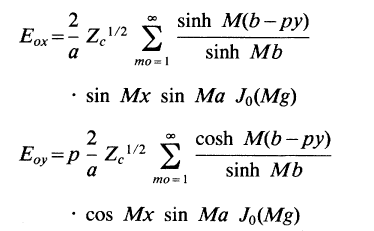
\includegraphics[width=0.5\linewidth]{DELETE.png}
    \caption{Normalized E field formula \cite{Wilson_Ma_1986}}
    \label{fig:placeholder}
\end{figure}

\begin{figure}[h]
    \centering
    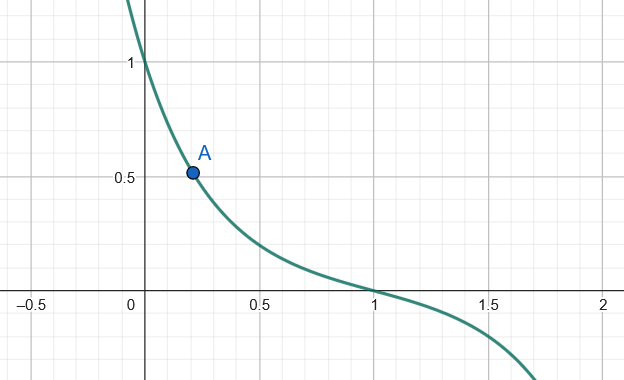
\includegraphics[width=0.5\linewidth]{DELETE2.png}
    \caption{Normalized e-field distribution along z-axis at center of septum}
    \label{fig:placeholder}
\end{figure}

\todo{The electric field / magnetic field distribution of the TEM mode must be known ($e_0$). Other mode distributions are neither available, nor necessary. Calculations to find these field distributions can be found in \cite{4091811}. This would also solve the problem with not being able to shift the location of the electric dipole moment. In \cite{Sreenivasiah_Chang_Ma_1981}, the normalized electric field was also determined analytically, just with output power. IMPORTANT!!! Additionally, the electric field at the output port and the dipole location must be equal (in tem mode) for the formula to work. If they are not, then the formulas derived in \cite{4091811} must be used. That's why the formula does not work for offset shift of the dipole moment anymore. The electric field at the incident port must then be found out. How to use this in case of a shielding material?}

% The paper goes on to talk about the total power radiated by the EUT in free space. I don't think I need that, but this comment is here as a reminder that it exists.

